%%%%%%%%%%%%%%%%%%%%%%%%%%%%
\documentclass[a4paper,11pt,spanish]{report}
%%%%%%%%%%%%%%%%%%%%%%%%%%%%
% LINE SPACING
\newcommand{\linespacing}{1.5}
\renewcommand{\baselinestretch}{\linespacing}
%%%%%%%%%%%%%%%%%%%%%%%%%%%%
%%%%%%%%%%%%%%%%%%%%%%%%%%%%
%BIBLIOGRAPHY STYLE
\usepackage{natbib}
\bibliographystyle{plain}
\makeatletter
\renewcommand\@biblabel[1]{}
\makeatother

% \bibliographystyle{plain} for [1], [2] etc.
%%%%%%%%%%%%%%%%%%%%%%%%%%%%

%%%%%%%%%%%%%%%%%%%%%%%%%%%%
% OTHER FORMATTING/LAYOUT DECLARATIONS
% Graphics
\usepackage{algorithm}
\usepackage[noend]{algpseudocode}
\makeatletter
\def\BState{\State\hskip-\ALG@thistlm}
\makeatother

\usepackage[noend]{algpseudocode}
\usepackage{graphicx,color}
\usepackage[english]{babel}
\selectlanguage{English}
\usepackage[utf8]{inputenc}
%\usepackage{listings}
%\lstset{language=Python}
\usepackage{amsmath}
\usepackage{microtype}
\usepackage{enumitem}
\usepackage{minted}
\usepackage{mdframed}
\usepackage{longtable}
\usepackage{booktabs}
\usepackage{epstopdf}
%\usepackage[british]{babel}
% The left-hand-side should be 40mm.  The top and bottom margins should be
% 25mm deep.  The right hand margin should be 20mm.
\usepackage[a4paper,top=2.5cm,bottom=2.5cm,left=2.7cm,right=2.5cm,headsep=10pt]{geometry}
%\flushbottom
% Pages should be numbered consecutively through the main text.  Page numbers
% should be located centrally at the top of the page.
\usepackage{fancyhdr}
\fancypagestyle{plain}{
	\fancyhf{}
	% Text in header
 	%\lhead{\textit{\today}}
	%
	\cfoot{\thepage}
	\renewcommand{\headrulewidth}{0pt}
}
% Paragraph separation and indents
\pagestyle{plain}
\setlength{\parskip}{\baselineskip}%
\setlength{\parindent}{0pt}
%%%%%%%%%%%%%%%%%%%%%%%%%%%%

%%%%%%%%%%%%%%%%%%%%%%%%%%%%
% HYPER REF
\usepackage[colorlinks,pagebackref,pdfusetitle,urlcolor=black,citecolor=black,linkcolor=black,bookmarksnumbered,plainpages=false]{hyperref}
% For print version, use this instead:
\usepackage[pdfusetitle,bookmarksnumbered,plainpages=false]{hyperref}
\usepackage{backref}
\renewcommand{\backrefpagesname}{Cited on}
\definecolor{light-gray}{gray}{0.98}
%%%%%%%%%%%%%%%%%%%%%%%%%%%%

%%%%%%%%%%%%%%%%%%%%%%%%%%%%
% BEGIN DOCUMENT
\begin{document}
\raggedbottom
%%%%%%%%%%%%%%%%%%%%%%%%%%%%

%%%%%%%%%%%%%%%%%%%%%%%%%%%%
% PREAMBLE: roman page numbering i, ii, iii, ...
\pagenumbering{roman}
%%%%%%%%%%%%%%%%%%%%%%%%%%%%

%%%%%%%%%%%%%%%%%%%%%%%%%%%%
%% TITLE PAGE: The title page should give the following information:
%%	(i) the full title of the thesis and the sub-title if any;
%%	(ii) the full name of the author;
%%	(iii) the qualification aimed for;
%%	(iv) the name of the University of Sussex;
%%	(v) the month and year of submission.
% \thispagestyle{empty}
% \begin{flushright}
% \includegraphics[width=6cm]{figures/LOGO_ESCUELA}
% \end{flushright}
% \vskip40mm
% \begin{center}
% % TITLE
% \huge\textbf{Development of unsupervised learning transformations through supervised learning methods.}
% \vskip2mm
% % SUBTITLE (optional)
% \LARGE\textit{}
% \vskip5mm
% % AUTHOR
% \Large\textbf{Author: Patricia Cortajarena Sauca}

% \Large\textbf{Ponente: Carlos Roberto del Blanco Adán}

% \Large\textbf{Tutor: Iñigo Cortajarena Sauca}

% \Large\textbf{Dep: GTI: Grupo de Tratamiento de Imágenes}

% \end{center}
% \vfill
% \begin{flushleft}
% \large
% QUALIFICATION
% Trabajo Fin de Grado.
% ETSIT UPM.
% % DATE OF SUBMISSION
% Madrid. January, 2018.
% \end{flushleft}
%%%%%%%%%%%%%%%%%%%%%%%%%%%%

%%%%%%%%%%%%%%%%%%%%%%%%%%%%
% ABSTRACT
\chapter*{Abstract}
\setcounter{page}{3}

Since dimensionality reduction has turned to be an important task in machine learning problems, the aim of this project is the development of a supervised machine learning embedding algorithm that seeks to replicate other algorithms' transformations such as MDS and t-SNE which are non-parametric and non-reusable. Moreover, since we are using a neural net to do so, ours can be re-used, reproduced and taken advantage of in a more efficient and convenient way. This algorithm can also be implemented for nearest neighbours search in a lower dimensional space obtained from the model.

The usage of real data-sets and neural nets are the main tools used for this study. The results obtained show the trade-off between precision, computational time and memory usage. The loss of precision of the model developed is negligible compared to the improvements in time and memory.

Keywords: \textit{Machine learning, unsupervised-learning, embedding, neural nets, dimensionality reduction, nearest neighbours.}

%%%%%%%%%%%%%%%%%%%%%%%%%%%%
% RESUMEN
\chapter*{Resumen}

Los algoritmos de reducción de dimensiones suponen un paso imprescindible en problemas de aprendizaje automático. Por ello, el objetivo de este proyecto es el desarrollo de un modelo supervisado de reducción de dimensiones que sea capaz de replicar las transformaciones que realizan otros algoritmos no paramétricos y no reutilizables como MDS o t-SNE. Además, al utilizar redes neuronales para llevarlo a cabo, conseguimos que nuestro modelo sea reutilizable, reproducible y sacar partido de ello de una forma eficiente. Asimismo, este modelo podría usarse para la obtención eficiente de vecinos cercanos en un espacio de menor dimensión obtenido a partir del mismo.

Las principales herramientas usadas para la investigación son bases de datos reales y redes neuronales. Los resultados obtenidos muestran una relación directa entre precisión y uso de tiempo y memoria. La pérdida de precisión es imperceptible en comparación con la mejora en tiempo computacional y uso de memoria.

Palabras clave: \textit{Aprendizaje automático, aprendizaje no supervisado, redes neuronales, redución de dimensiones, vecinos cercanos.}

%%%%%%%%%%%%%%%%%%%%%%%%%%%%
% ACKNOWLEDGEMENTS
\chapter*{Acknowledgements}

Special thanks to my director, Carlos Roberto del Blanco Adán, for his professional guidance, enthusiastic encouragement and priceless help. Thanks to my family for their unconditional support and to my tutor Iñigo Cortajarena Sauca for introducing me to the world of machine learning, for his constructive recommendations and for his valuable technical help on this project.

\renewcommand{\baselinestretch}{\linespacing}
\small\normalsize
% ACKNOWLEDGEMENTS HERE:
%%%%%%%%%%%%%%%%%%%%%%%%%%%%%

%%%%%%%%%%%%%%%%%%%%%%%%%%%%%
% TABLE OF CONTENTS, LISTS OF TABLES & FIGURES
\newpage
\pdfbookmark[0]{Contents}{contents_bookmark}
\tableofcontents
\listoftables
\phantomsection
\addcontentsline{toc}{chapter}{List of Tables}
\listoffigures
\phantomsection
\addcontentsline{toc}{chapter}{List of Figures}
%%%%%%%%%%%%%%%%%%%%%%%%%%%%%

%%%%%%%%%%%%%%%%%%%%%%%%%%%%%
% MAIN THESIS TEXT: arabic page numbering 1, 2, 3, ...
\newpage
\pagenumbering{arabic}
%%%%%%%%%%%%%%%%%%%%%%%%%%%%%

%-----------------------------------------------------
% Chapter: Introduction
%-----------------------------------------------------

\chapter{Introduction}
\label{chap:intro}

Working with large datasets and high-dimensional data in nowadays' problems has encouraged the use of dimensionality reduction algorithms which try to preserve as much information as possible even with a reduced number of features used to describe that same dataset. This is, dimensionality reduction algorithms compute new features based on the original ones. Although the number of new features computed are less than the number of original ones, the reduction's objective is to still represent the same information without significant distortion. Thus, time and memory may be saved when facing large implementations.

Taking into account that this turns into a difficult task, numerous approaches have been proposed.
Although the different approaches try to achieve more or less the same aim, they differ from one another and we can not reassure which one would suite a specific problem or even if the behaviour of the algorithm throws the results we expected or needed.

The first point to take into account is the existence of parametric and non-parametric algorithms, depending on whether the dimensionality reduction can be expressed in terms of parameters or not, which can be conclusive when deciding what algorithm to use. Secondly, in both of them we can find different models proposed depending on what to optimize, yet not everything is going to be preserved as well as in the original dataset, so we need to prioritize some aspects.

The decision of which of them to implement depends on the previous study of our data, the performance requirements and the later purpose and usage of the embedded data.

Non-parametric algorithms have an important disadvantage: as previously said, they don't have parameters which represent the dimensionality reduction transformation; thus, when a new sample is provided we need to compute the whole algorithm again to obtain the data point's coordinates in the lower dimensional space, instead of computing the transformation on this sample alone. This is computationally expensive and somewhat inconvenient for real world applications.

We hereby propose the study and research an implementation of a machine learning model which can replicate the behaviour of a non-parametric dimensionality reduction algorithm. The main objective is to resolve the latter's main disadvantage and make it capable of being repeatedly used with new examples, omitting the need to compute the whole non parametric transformation every time, saving time and computational resources.

The embedding algorithms used as a baseline for this research are the ones listed below:

\renewcommand{\labelitemi}{\textendash}
\begin{itemize}
\item PCA (Principal Component Analysis)
\item MDS (Multidimensional Scaling)
\item TSNE (T-Stochastic Neighbour Embedding)
\end{itemize}

These algorithms have been selected for different reasons. Firstly, PCA is known to be the basic linear model on which MDS relies, it is widely used (mainly to eliminate correlation issues and as a general compression algorithm) and accepted for real applications for its relative simplicity and interpretability. MDS is capable of preserving distances, both euclidean and geodesic, which means that it could be applied in applications that depend on this, such as nearest neighbours search or clustering. Lastly, t-SNE is a state-of-the-art algorithm when looking at preserving both local and global structure of the data, and is often used for visualizations or even as a feature engineering trick.

To conclude, the document is divided into chapters which summarize the main steps of this research. Chapter number \ref{chap:stt} describes the State-of-The-Art. It is followed by chapter \ref{chap:frame}, which details the main steps of the implementation and describes the main implementation's applications and the corresponding metrics computed to analyze the algorithm's behaviour. The next chapter (chapter \ref{chap:conc}) comprehends the conclusion and summarizes the main ideas discussed in this paper. Finally, chapter \ref{chap:appendix} includes the code implemented to carry out the research.

%-----------------------------------------------------
% Chapter: State of the Art
%-----------------------------------------------------

\chapter{State-of-The-Art}
\label{chap:stt}

Two of the most classical dimensionality reduction techniques are know to be PCA \citep{pca} and MDS \citep{mds}. They try to preserve the true structure of the data even though they are simple to implement and computationally efficient. They rely on linear models to compute an embedding of the original space into a lower dimensional one. A related linear implementation which is based on random projections of the data is described in \citep{rproj, rproj2}. Some other well-known techniques are ISOMAP \citep{isomap} and t-SNE \citep{tsne}, but their implementations often require more memory and computational load, yet the complexity of the algorithms is higher. Nevertheless, these algorithms are capable of reducing the number of features in a non-linear manner, whereas linear models can not faithfully represent the data's structure since the output space's coordinates must always be linear combinations of the original features. ISOMAP computes geodesic distances instead of euclidean dissimilarities while t-SNE's approach is to compute probabilities from an euclidean metric.

Neural networks have become an essential tool in machine learning problems and can certainly be used for dimensionality reduction. Autoencoders \citep{auto2, auto} consist on a neural net with a  decreasing number of neurons per layer and a symmetrical structure whose output's size is the same as the input's. If the output represents the input without any distortion, then middle layer with the fewest number of neurons corresponds to the embedded description of the data. This is represented in figure \ref{autoencoder}.

\begin{figure}[h]
\centering
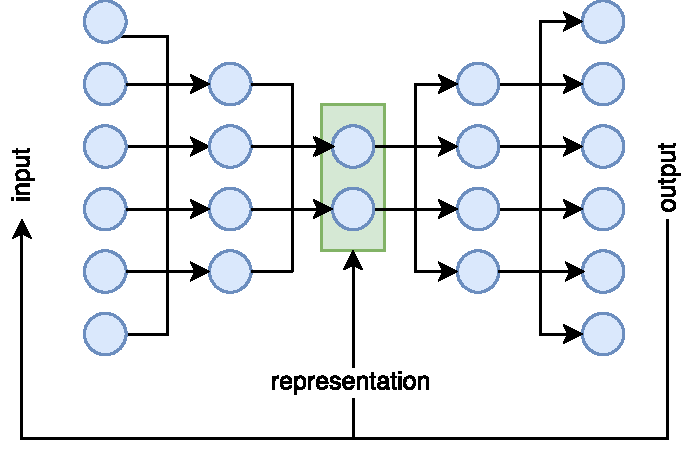
\includegraphics[width=8cm]{figures/autoencoder.pdf}
\caption{\label{autoencoder}Autoencoder neural network.}
\end{figure}

The following sections (sections \ref{sec:pca}, \ref{sec:mds} and \ref{sec:tsne}) summarize the main ideas of the algorithms on which the research is based. 

\section{PCA: Principal Component Analysis}
\label{sec:pca}

Principal Component Analysis \citep{pca} is based on reducing the number of features by processing the correlations amongst them. The aim is to eliminate these correlations by representing the matrix \textbf{X} $\in$ $\Re^{mxn}$ (with m being the number of data points and n de number of features) in a lower dimensional orthogonal basis. By omitting the correlation between columns of the matrix \textbf{X} we are capable of doing away with redundancies.

The model starts by computing de covariance matrix, which results in a $\Re^{nxn}$ symmetric matrix by using the next expression:
\begin{center}
cov(\textbf{X}) = $\dfrac{1}{m-1}$ $\textbf{X}^{T}$\textbf{X}
\end{center}
Since the aim of the PCA is to eliminate the correlations, the covariance matrix of the resulting \textbf{Y}, corresponding to the matrix of the sample's coordinates in the lower dimensional space; should be a diagonal matrix with just the variances of the columns.

PCA is often used because of a great advantage: with it, a linear transformation \textbf{P} between the matrices of the high and low dimensional space (\textbf{Y = XP}) can be inferred. As the resulting transformation is basically a change-of-basis (matrix multiplication), it turns to be easy to reuse and computationally simple in those cases where the number of samples is moderate, yet the computational complexity of this algorithm is quadratic with the number of them: $O(N^{2})$.

For any symmetric matrix we can find an eigenvalue decomposition to a diagonal matrix, matching exactly our problem (with \textbf{X} and \textbf{Y} and their covariances) \citep{pca}.

\begin{center}
\textbf{Y = XP}
$$ cov(\textbf{Y}) = \frac{1}{m-1} \textbf{Y}^{T} \textbf{Y} = \frac{1}{m-1} \textbf{(XP)}^{T} \textbf{XP} = \textbf{P}^{T} cov(\textbf{X})\textbf{P} $$
$$\textbf{D} = \textbf{V}^{T} \textbf{AV}$$
$$ \textbf{A} = cov(\textbf{X}); \textbf{P} = \textbf{V}^{T}; \textbf{D} = cov(\textbf{Y})$$
\end{center}

With the previous expressions we get to the point that, by computing the eigenvectors of the covariance matrix \textbf{X}, we can get a linear transformation from space \textbf{X} to space \textbf{Y}. The matrix of eigenvalues obtained (cov(\textbf{Y})) are sorted decreasingly and the vectors of the orthogonal basis. Choosing the \textbf{N} first values of this matrix, being \textbf{N} the desired output dimension, and computing the corresponding change-of-basis, we obtain the coordinates of the samples in the output space.

\section{MDS: Multidimensional Scaling}
\label{sec:mds}

Multidimensional Scaling \citep{mds} is a dimensionality reduction technique that tries to create a map which preserves the relative distances between the data points. This lower dimensional embedding aims to keep as much distance information as possible. In order to visualize data, this dimensional map needs to be a one, two or, at most, three dimensional space.

MDS computes a metric or non-metric solution depending on the input matrix provided, which has to be a \textit{proximity} matrix. This \textit{proximity} matrix quantifies how close the samples are in the original space. On the one hand for metric solutions, this \textit{proximity} matrix has to be a true distance matrix, while on the other, both dissimilarities or correlations are alternatives to the input for the problem's matrix. Since computations between all of the samples in both of the cases are needed (distances or proximity matrix computation), this algorithm turns to be of  quadratic order with the number of them: $O(N^{2})$.

MDS algorithm is based on some ideas discussed in the previous section. The \textit{proximity} matrix is always  symmetric and somehow describes the relations between the features. This means that we can basically treat our problem as a variation of the PCA algorithm.

Metric MDS performs the same steps as in PCA, being a distance matrix the input to the algorithm.

In non metric MDS, we assume a less strict relation and we compute the observed distances as a function of the real distance plus some measure error. The usable information in this case is going to be the rank order of the previous matrix, which could be the input for the model.

The main difference between PCA and MDS is the fact that, because of the need to compute a pairwise distance or proximity matrix, there is no linear transformation that suits both the distance computations plus the matrix operations (PCA / change-of-basis), so MDS turns to be non-parametric.

\subsection{Loss function: Stress}
\label{ssec:str}

In every machine learning problem, we need a loss function which quantifies how well the algorithm is fitting our data. This loss function can be convex or not, but in any case it will have to be optimized by the algorithm (either majorized or minimized). In Multidimensional Scaling we compute the \textit{stress} loss function that compares the distances in the output space with the original ones. Note that this obviously depends on the number of dimensions we want to keep; if we lower the number of dimensions, the stress will be higher since we are trying to represent the same distance relations in a smaller number of dimensions.

\begin{center}
\( \textit{stress} = \sqrt{\frac{\sum(d_{ij}-d'_{ij})^{2}}{\sum d_{ij}^{2}} } \)
\end{center}

$d_{ij}$ represents the original distance and $d'_{ij}$ is the distance in the output space (based on the MDS model). This last value is either a predicted true distance or a function which represents the non-metric transformation of the data.

Regarding the previous expression, if our prediction stands well for the original data, the stress value should be lower, relating zero stress to the perfect performance of the MDS  algorithm.

\section{TSNE: T-Stochastic Neighbour Embedding}
\label{sec:tsne}

T-Stochastic Neighbour Embedding \citep{tsne} is an example of a non-linear dimensionality reduction algorithm. It relies on Stochastic Neighbour Embedding (SNE). The main reason why this method is used is because it is capable of representing both the local and the global structure of the original data. This section will be divided in two: the basis SNE and the t-SNE upgrades.

\subsection{SNE}
\label{ssec:sne}

SNE approaches the dimensionality reduction by converting the Euclidean distances into conditional probabilities as a way of expressing similarities between points. This means that we measure the similarity of two points $x_{i}$, $x_{j}$ as the probability $p_{i|j}$ of finding the second one as a neighbour of the first. For the lower dimensional similarity, the probability $q_{i|j}$ would be obtained similarly but with the low-dimensional coordinates instead. Thereby, the probability in the original and in the low dimensional space is computed as seen \citep{tsne}:

$$ p_{i|j} = \frac{exp(-||x_{i}-x_{j}||^{2}/2\sigma_{i}^{2})}{\sum _{k\neq i} exp (-||x_{i}-x_{k}||^{2}/2\sigma_{i}^{2})}$$

$$ q_{i|j} = \frac{exp(-||y_{i}-y_{j}||^{2})}{\sum _{k\neq i} exp (-||y_{i}-y_{k}||^{2})} $$

These expressions represent probabilities under gaussian distributions centered in each datapoint $x_{i}$, where $\sigma_{i}$ is the sample's variance. The conditional probability represents how likely it is for the point $x_{j}$ to be considered a sample's neighbour. According to the value of $\sigma_{i}$ the probabilities change, so it is chosen depending on the density of the data. In a dense region, a smaller value of $\sigma_{i}$ is more appropriate than in a sparse region. Having decided which value to use for each of the samples, we obtain a probability distribution, $P_{i}$, that is computed as explained in the next paragraph.

As the point of this metric is to compute similarities as probabilities, we can calculate the mismatch between $p_{i|j}$ and $q_{i|j}$ for all the samples and consequently obtain the algorithm's behaviour by analysing how many neighbours have been kept in the low dimensional map. In terms of conditional probabilities, Kullback-Leibler divergence perfectly suits this need. Summing up all the previous ideas we get to the point of minimizing the cost function described as \citep{tsne}:

$$ C = \sum\limits_{i} KL(P_{i}||Q_{i}) = \sum\limits_{i} \sum\limits_{j} p_{i|j} log \frac{p_{i|j}}{q_{i|j}}$$

The limitations of this algorithm are the non symmetric general expression of the Kullback-Leibler divergence, the difficulty to optimize the cost function, the fact that we need to choose different values of the variance depending on the point and the "crowding problem". T-SNE tries to solve these limitations.

\subsection{t-SNE}
\label{ssec:tsne}

Although SNE is capable of showing good visualizations and is widely accepted, t-SNE was proposed as a modification to this algorithm which tried to make it more accurate and lower its computational cost.

Instead of minimizing the sum of the different KL divergences along all the samples, another way of computing the cost is proposed: we are trying to minimize a single KL divergence between a joint probability P and the equivalent one in the low dimensional space, Q. With this symmetric approach, we omit the need to obtain the variances for each sample and the cost function is much easier to compute and optimize, and so is its gradient \citep{tsne}.

$$ C = KL(P||Q) = \sum\limits_{i} \sum\limits_{j} p_{ij} log \frac{p_{ij}}{q_{ij}}$$

$$ \frac{\partial C}{\partial y_{i}} = 4 \sum\limits_j (p_{ij} - q_{ij}) (y_{i} - y_{j}) $$

Moreover, t-SNE handles the problem known as "crowding problem" extremely well by introducing a heavy-tailed distribution, the Student-t distribution, rather than a Gaussian for the low-dimensional space. The "crowding problem" appears when we want to faithfully represent mutually equidistant points while going from a high-dimensional space to low-dimensional one. This task tends to be quite difficult because the area / volume available in a lower dimensional space is considerably smaller than in the high dimensional one. In the end, the points tend to clash in the center of the map, and it becomes hard to represent and preserve the true distances from the original space.

The t-Student distribution is a heavy-tailed distribution and it allows for a more faithful representation of distances. The joint probabilities are now then computed as follows:

$$ q_{ij} = \frac{(1+ ||y_{i}-y_{j}||^2)^{-1}} {\sum\limits_{k\neq l} (1+ ||y_{k}-y_{l}||^2)^{-1} }$$

The reason why this particular distribution was chosen is because it is closely connected to the Gaussian distribution, as the t-Student is an infinite mixture of Gaussians.

To conclude, the gradient of the Kullback-Leibler divergence taking into account these changes in the Q low-dimensional space stands for the next expression:

$$ \frac{\partial C}{\partial y_{i}} = 4 \sum\limits_j (p_{ij} - q_{ij}) (y_{i} - y_{j}) (1+ ||y_{i}-y_{j}||^2)^{-1}$$

\section{Supervised Learning Algorithms: Neural nets and Decision Trees}
\label{supervised}

Two main supervised learning algorithms used in today's applications are Neural Networks and Decision Trees. To know which of them or even if both could suit our problem we studied their main characteristics and differences.

First of all, decision trees are believed to be faster and easier to train, and their results can be very interpretable. On the other hand, neural nets are slower to train (not so with GPUs) and less interpretable (usually considered black-boxy). Neural networks are prone to over-fitting if the size of the given data-set is not large enough or if the parameters used for regularization aren't the best for a particular use case, while decision trees are less prone to over-fitting if correctly pruned / regularized (eliminating some of the tree's branches and restricting tree depth can help to mitigate these issues). What really makes the difference from one another is the fact that neural nets are capable of having two or more output variables (when considering general regression) while the regression trees can only handle one output. Whenever decision trees need to be used for multi-output regression, multiple trees are needed, which increases computational complexity and performance assessment, since each of the trees / tree models may have different hyper-parameters.

Taking these differences into account, the supervised learning algorithm chosen for this research is neural networks, since it is a flexible and powerful tool that can learn smooth mathematical functions but also complex non-linear and possibly noisy relationships. The advantage of our framework relies on the fact that, as it's said, due to being a supervised algorithm, it is possible to reuse it after the training process since the parameters and weights of the net can be stored.

%-----------------------------------------------------
% Chapter: Framework
%-----------------------------------------------------

\chapter{Framework}
\label{chap:frame}

\section{General framework}
\label{gframe}

We hereby propose the implementation of a supervised learning tool which learns the embedding derived by an unsupervised learning method, which could be used in real machine learning applications.

Multidimensional Scaling and T-Stochastic Neighbour Embedding are both non-parametric dimensionality reduction algorithms. As it was discussed in the introduction (Chapter \ref{chap:intro}), these algorithms are not parametric and  non-reusable; once the embedding is computed, if we wanted to add a new sample to the dataset and obtain its embedded vector, we would need to compute everything again in order to include the new sample, which may lead to different results and implies a huge amount of computation. This is impractical and not suitable for real life applications.

Having said that, we have a set of \textbf{m} samples with \textbf{n} features each, and we want to represent those points in a lower-dimensional space, for which we are willing to use a neural net (supervised algorithm) which can learn that embedding, replicating any of the previously mentioned dimensionality reduction algorithms (unsupervised, non-parametric and gradient descent based).

The neural network model (chosen as the suitable model for our applications \ref{supervised}) needs to be trained at least once, so we need to first compute the dimensionality reduction algorithm (step 1, figure \ref{figurenet}) to feed the results into the neural net with its output being the reduced vectors computed by the latter. Having the neural net trained and its weights stored (step 2, figure \ref{figurenet}), as we get a new sample, instead of recalculating the MDS or the t-SNE from scratch, we can reuse the neural net's parameters to obtain a prediction (step 3, figure \ref{figurenet}) which is the lower dimension vector of this sample.

With this implementation we are able to speed up the process, reduce memory usage (since we only need to store the neural net's weights) and also reduce computational time considerably.

\vspace{25px}

\begin{figure}[h]
\centering
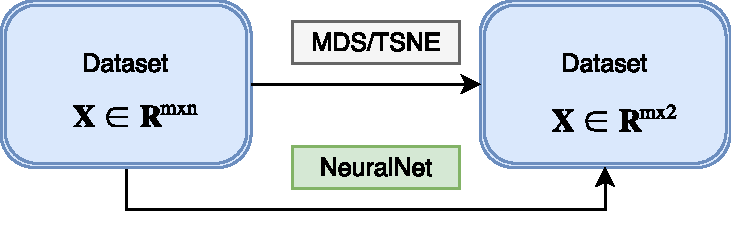
\includegraphics[width=12cm]{figures/neuralnet.pdf}
\caption{\label{figurenet}Dimensionality reduction algorithm learned by a Neural Network}
\end{figure}

\subsection{Cross Validation}
\label{sec:cv}

Cross validation is a technique used to evaluate predictive models and its aim is to estimate if the model is capturing the general or underlying structure of the data and can suit new unseen examples, and also estimate how accurate the model is only taking into account these unseen samples (in-sample performance is useless since the training set can be easily over-fitted with a complex enough model).

The easiest way to know whether a model is under-fitting or over-fitting is dividing the dataset into training set and test set, choosing for example 80\% to train the model and 20\% to test its behaviour in samples that have not been seen yet. Although this is a good first approach, we might be fitting our model to the test samples by trial and error without noticing it; this is, we might be choosing the model's parameters to fit the test set, and still not capturing the overall underlying function of the data-set.

A more robust approach would be to use cross validation, which consists in dividing the data into a number of disjoint folds; some usual choices are  three, five  and ten folds, where this choice depends only on the size of the dataset (smaller datasets usually require larger number of folds). The algorithm is then trained repeatedly, choosing every time one of the folds to test and the rest of them to train. As we have trained and tested the model with disjoint samples, we are not fitting our model to certain subsets of the dataset. We use an error metric to the model's performance in all test / validation folds and compute the mean and variance of this error metric along all folds. The mean represents the expected performance in a future live test (always considering that the underlying problem or dynamics don't change, an issue that may happen in real live situations) and the standard deviation of the error throughout all folds is a measure of model variance. High deviations may imply that the model is over-fitted (overly complex) and that we may need to regularize it more. The best cross validation performance usually comes from a correct balance between bias and variance for our model, which comes from a correct choice of hyper-parameters. The following schema represents the cross validation procedure.

\vspace{25px}

\begin{figure}[h]
\centering
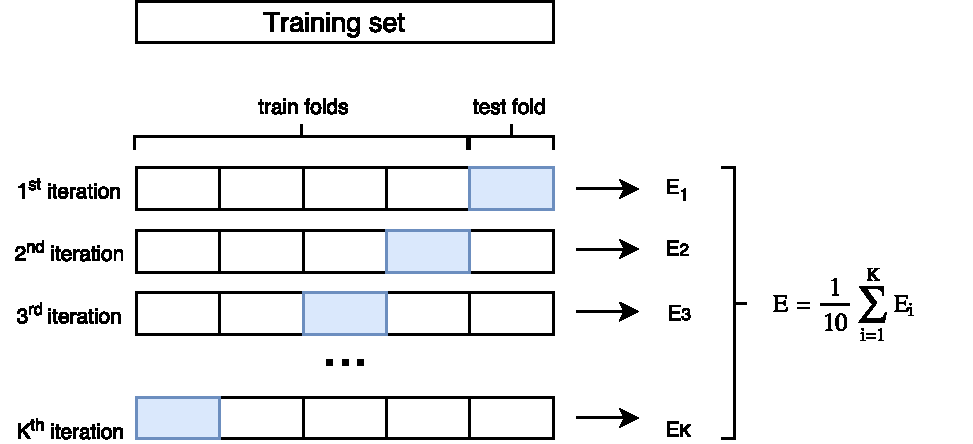
\includegraphics[width=15cm]{figures/cv.pdf}
\caption{\label{figurefit}Cross validation using K-Folds.}
\end{figure}

\section{Framework 1: Replicating t-SNE/MDS with neural net}
\label{sec:app1}

The first implementation to be discussed is the base model to replicate a general non-parametric dimensionality reduction algorithm. For this particular use case, T-Stochastic Neighbour Embedding and MDS are used as the algorithms to carry out transformations with. The main objective is to assess whether the supervised neural net is capable of replicating the previous algorithms.

\subsection{Algorithm: t-SNE/MDS and neural net}
\label{ssec:dra}

This section discusses the computation of the space reduction algorithm and the supervised replicator implementation using a neural net model (algorithm \ref{alg1}).

As a starting point for the problem, the embedding model is computed for all the data points beforehand. These values obtained are the ground truth labels for the training phase. Standardization is carried out for all features in the original data by removing the mean and scaling to unit variance. This is done for each of the 64 variables, since the neural net is sensible to scales. We don't do the scaling inside cross validation since our only aim is to check whether the neural net can learn the space mapping or not, so this is completely different to usual machine learning problems; our output here is the sample vectors / embeddings derived from the unsupervised model. Due to the data set containing 1797 instances with 64 features each, a two dimensional space output is chosen, in order to be able to visualize the results.

Once the embeddings are obtained, both the original and the compressed samples are divided into two corresponding folds, one for training the neural net and the other one to test whether the model can correctly locate unseen points where the unsupervised model had placed them. The results obtained from the testing phase are shown in \ref{ssec:met1}. Therefore, by doing this, we are actually able to check if the neural net is capturing the general behaviour of the dimensional reduction algorithm and can replicate it further on.

To continue, the next to consider is the neural net's structure.  There are several kinds of neural nets depending on their topology. The main structure parameters for a neural net with no convolution or pooling (simple perceptron-like structure) are the number of layers, the number of neurons per layer, dropout, activation function, optimizer... Since the transformation or mapping function derived by the unsupervised method seems to be pretty smooth (complex but with low noise levels), low regularization (no $L2$) with no dropout, in combination with adagrad optimizer and hyperbolic tangent activation function; threw the best results. Depending on these a neural network can be shallow or deep (number of hidden layers) and wide or narrow (neurons per layer). Depending on the kind of structure used, the results obtained will differ from one another. In section \ref{ssec:met1} the differences between them are shown.

Taking into account that the aim of this first application is to replicate unsupervised learning and non-parametric algorithms, the neural nets designed do not use convolutions or pooling even though the dataset is made of images. As a general approach and taking into account the fact that these algorithms' gradient descent operates directly over raw features and learn non-linear functions to transform these directly into embedding vectors, there is no need to compute convolutions or pooling. As these transformation functions are smooth, the dense-like neural structure used performs well (as shown afterwards) and is able to learn these functions adequately. Also, this approach is generalizable to any machine learning problem no matter the kind of features or unsupervised algorithm used.

Once the net is built, the standardized original data from the training subset will constitute the net's input in the training process. The output is, in our case, a two variable output, and corresponds to the coordinates of all embeddings. The decision of choosing two variable output is to be able to visualize the results obtained. Nevertheless in the next application a comparison between different dimensions embeddings is done.

The neural net aims to get the same output as the dimensionality reduction algorithm, that is why the loss function used for the neural net's gradient descent is the Mean Squared Error euclidean distance error metric (MSE, although this is not the only possible loss function). This way, the neural net tries to minimize the distance between the true position obtained directly from t-SNE or MDS and the position being predicted by the model. In this case the distance metric that throws the best overall results corresponds to the mean of the euclidean distances between true and predicted locations. Other metrics were also tested, such as mean loss (mean of the square of the difference between points) but results were not as good. The following equation describes the loss function used (where $n$ represents samples and $j$ dimensions):

$$ e = \frac{\sum^{n}{\sqrt{\sum^j{{(\hat{y}}}_{j} - y_{j})^{2}}}}{n} $$

To conclude, as the net has been trained to obtain two output values depending on the 64 feature standardized values in the input, it is possible to predict, taking into account the new input, the embedded data replicating what the non-parametric embedding model would compute, but avoiding the need to recalculate the whole algorithm.

\vspace{25px}
\begin{algorithm}
\caption{neural net replicating process}
\label{alg1}
\begin{algorithmic}[1]
\Procedure{Replicating Procedure}{}
\BState \emph{data obtaining}
\State $\textit{\textbf{X}} \gets \text{standardized input matrix}$
\State $\textit{\textbf{X\_emb}} \gets \text{compute t-SNE/MDS from \textit{\textbf{X}}}$
\State $\textit{\textbf{X\_train; }} \textit{\textbf{X\_test; }} \textit{\textbf{X\_emb\_train; }} \textit{\textbf{X\_emb\_test; }}  \gets \text{train and test data computation}$
\BState \emph{neural net model construction}
\BState \emph{fit neural net model}
\State $\textit{\textbf{X\_train}} \gets \text{neural net's input}$
\State $\textit{\textbf{X\_emb\_train}} \gets \text{neural net's output}$
\State $\textit{\textbf{distance error}} \gets \text{neural net's error metric}$
\BState \emph{predict neural net model}
\State $\textit{64 feature input (new example)} \to \text{neural net} \to \text{predict output = } \text{\underline{dimension reduction}}$
\EndProcedure
\end{algorithmic}
\end{algorithm}

\subsection{Results}
\label{ssec:res1}

\begin{itemize}
    \item Dataset
\end{itemize}
The dataset \textit{"load-digits"} is the data used to test this example and is obtained from the Scikit-Learn datasets \citep{scikit-learn}. It consists of 1797 instances of handwritten digits from 0 to 9 from different writers with 64 features each. This features represent the values of gray-scale intensity for each pixel in the image. Our images are 8x8 pixel images represented by  a total of 64 features with a color resolution (brightness in case of grey-scale) ranging from 0 (completely black) to 16 (pure white) as show in figure \ref{figuredigit}. To translate this into a training set, each image is flattened as a row with its corresponding 64 pixel features; a last column with the label of the number represented in the image is concatenated to the table.

\begin{figure}[h]
\centering
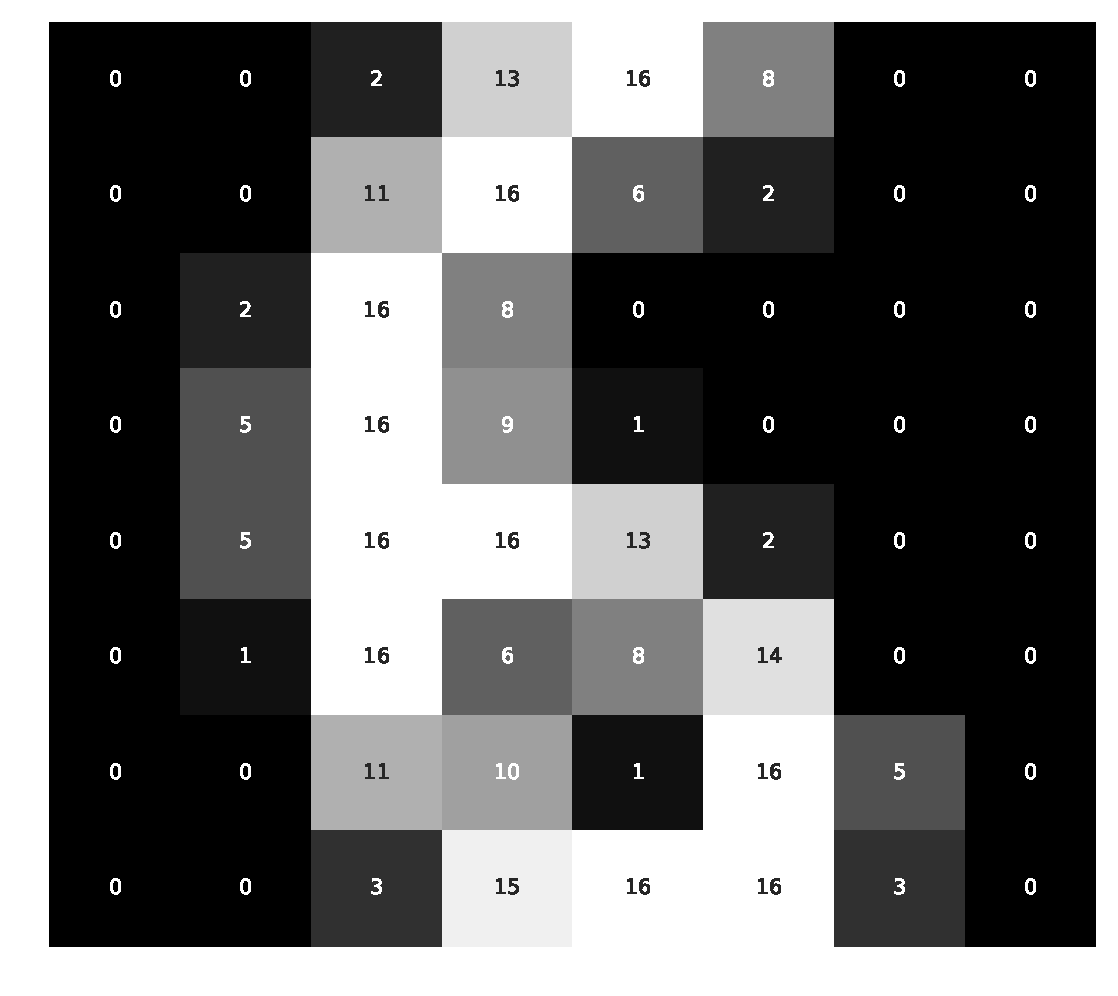
\includegraphics[width=9cm]{figures/exampledigit.pdf}
\caption{\label{figuredigit}Example dataset point representing a handwritten digit.}
\end{figure}

\begin{itemize}
    \item Metrics
    \label{ssec:met1}
\end{itemize}
The aim of this first implementation is not only to be able to reuse the embedding function but also to make if extremely CPU efficient to compute the location (reduced vector) of new samples and also provide a memory efficient way of doing this (we only need to store the neural net weights). 

To do this, several neural net structures were tested. For all neural net structures, transformation times and errors were computed in the following tables (tables \ref{metrics1}, \ref{metrics2}, \ref{times1} and \ref{times2}).

Recall that these measurements are performed over samples from the test set which are unseen for the model (non present during training), and thus they indicate the general behaviour of the model.

Tables \ref{metrics1} and \ref{metrics2} include the models' structures and the errors obtained for both of the embedding algorithms. As stated before, the model's structure depends on the total number of hidden layers, the number of neurons per layer and on the dropout applied to each layer (in the end no dropout was used as discussed before). The neural net structure is inherent in the length of the array in the table, where the length represents the number of layers. To summarize, the types of neural nets tested are divided into deep or shallow and wide or narrow nets.

The out of sample error computed is again an euclidean distance error and matches the loss function exactly. As stated before, it evaluates the difference between the position computed by t-SNE or MDS and what the model is predicting. The error value corresponds to the mean of these Euclidean distances. Percentages are also included to reckon whether the total error compared to the range of values acquired by the algorithms stand for a decent figure.

\begin{table}[p]
\vspace{20px}
\centering
\begin{tabular}{llllrrr}
\toprule
{} &       dropout &             layers &              type &     error &  \%error\_X &  \%error\_Y \\
\midrule
model1 &  [0, 0, 0, 0] &    [32, 16, 16, 8] &     deep - narrow &  6.335186 &  4.976027 &  5.882600 \\
model2 &        [0, 0] &           [32, 32] &  shallow - narrow &  5.810866 &  4.564196 &  5.395738 \\
model3 &        [0, 0] &           [32, 16] &  shallow - narrow &  6.276359 &  4.929821 &  5.827976 \\
model4 &     [0, 0, 0] &      [128, 64, 64] &       deep - wide &  3.379963 &  2.654821 &  3.138498 \\
model5 &  [0, 0, 0, 0] &  [128, 64, 64, 32] &       deep - wide &  3.481527 &  2.734596 &  3.232807 \\
model6 &     [0, 0, 0] &    [128, 128, 128] &    shallow - wide &  3.239071 &  2.544157 &  3.007672 \\
model7 &        [0, 0] &          [128, 64] &    shallow - wide &  4.151196 &  3.260593 &  3.854634 \\
model8 &           [0] &             [1000] &   shallow - wider &  5.510108 &  4.327962 &  5.116465 \\
\bottomrule
\end{tabular}

\caption{\label{metrics1}Comparison between model's errors obtained out of sample (t-SNE)}
\end{table}

\begin{table}[p]
\vspace{20px}
\centering
\begin{tabular}{llllrrr}
\toprule
{} &       dropout &             layers &              type &     error &  \%error\_X &  \%error\_Y \\
\midrule
model1 &  [0, 0, 0, 0] &    [32, 16, 16, 8] &     narrow &  1.539260 &  3.164186 &  2.495089 \\
model2 &        [0, 0] &           [32, 32] &  narrow &  1.434994 &  2.949851 &  2.326077 \\
model3 &        [0, 0] &           [32, 16] &  narrow &  1.401265 &  2.880517 &  2.271405 \\
model4 &     [0, 0, 0] &      [128, 64, 64] &       wide &  1.328322 &  2.730571 &  2.153166 \\
model5 &  [0, 0, 0, 0] &  [128, 64, 64, 32] &       wide &  1.238499 &  2.545926 &  2.007566 \\
model6 &     [0, 0, 0] &    [128, 128, 128] &    wide &  1.227050 &  2.522390 &  1.989007 \\
model7 &        [0, 0] &          [128, 64] &    wide &  1.257435 &  2.584852 &  2.038261 \\
model8 &           [0] &             [1000] &   wider &  1.557930 &  3.202565 &  2.525353 \\
\bottomrule
\end{tabular}

\caption{\label{metrics2}Comparison between model's errors obtained out of sample (MDS)}
\end{table}

Taking an in depth look at computation times and considering that neural nets' whole transformation consists in matrix scalar multiplications and parametric activation functions that can be also vectorized (hyperbolic tangent in our case), this allows for an extremely efficient computation of inferred coordinates (low CPU usage, high speed).

Tables \ref{times1} and \ref{times2} show the huge difference between the computational time (in seconds) of the dimensional reduction algorithm and the neural net's development for the same number of points, referring to the whole data set (1787 points in total).

\begin{table}[h]
\centering
\begin{tabular}{lr}
\toprule
{} &      times \\
\midrule
tsne   &  49.129993 \\
model1 &   0.132459 \\
model2 &   0.111072 \\
model3 &   0.130287 \\
model4 &   0.175929 \\
model5 &   0.190567 \\
model6 &   0.227528 \\
model7 &   0.211757 \\
model8 &   0.252915 \\
\bottomrule
\end{tabular}

\caption{\label{times1}Computational times (t-SNE)}
\end{table}

\begin{table}[h]
\centering
\begin{tabular}{lr}
\toprule
{} &      times \\
\midrule
unsup  &  28.104550 \\
model1 &   0.067040 \\
model2 &   0.082692 \\
model3 &   0.087886 \\
model4 &   0.089499 \\
model5 &   0.105532 \\
model6 &   0.133000 \\
model7 &   0.126438 \\
model8 &   0.184579 \\
\bottomrule
\end{tabular}

\caption{\label{times2}Computational times (MDS)}
\end{table}

\subsection{Conclusion}
\label{ssec:conc1}

After all and given the results shown in the previous tables, we can assure that, even ignoring the neural nets' diverse structures, all of them are certainly quicker in obtaining the embeddings. If we look for accuracy, a wide neural net is better at replicating both the t-SNE and MDS algorithms. In particular, the model 6 suits the best all problems presented.

The next four figures show the results obtained. The first and third ones represent the predictions from the neural networks of the location of all samples in the out-of-sample test for the best of the models in both problems (model 6), and the second and fourth ones represent the same points from the embedding algorithms (t-SNE and MDS). As it can be clearly seen, the neural net is able to faithfully replicate the position of new points and performs extremely well in terms of preserving the local structure of the dataset.

\begin{figure}[p]
\centering
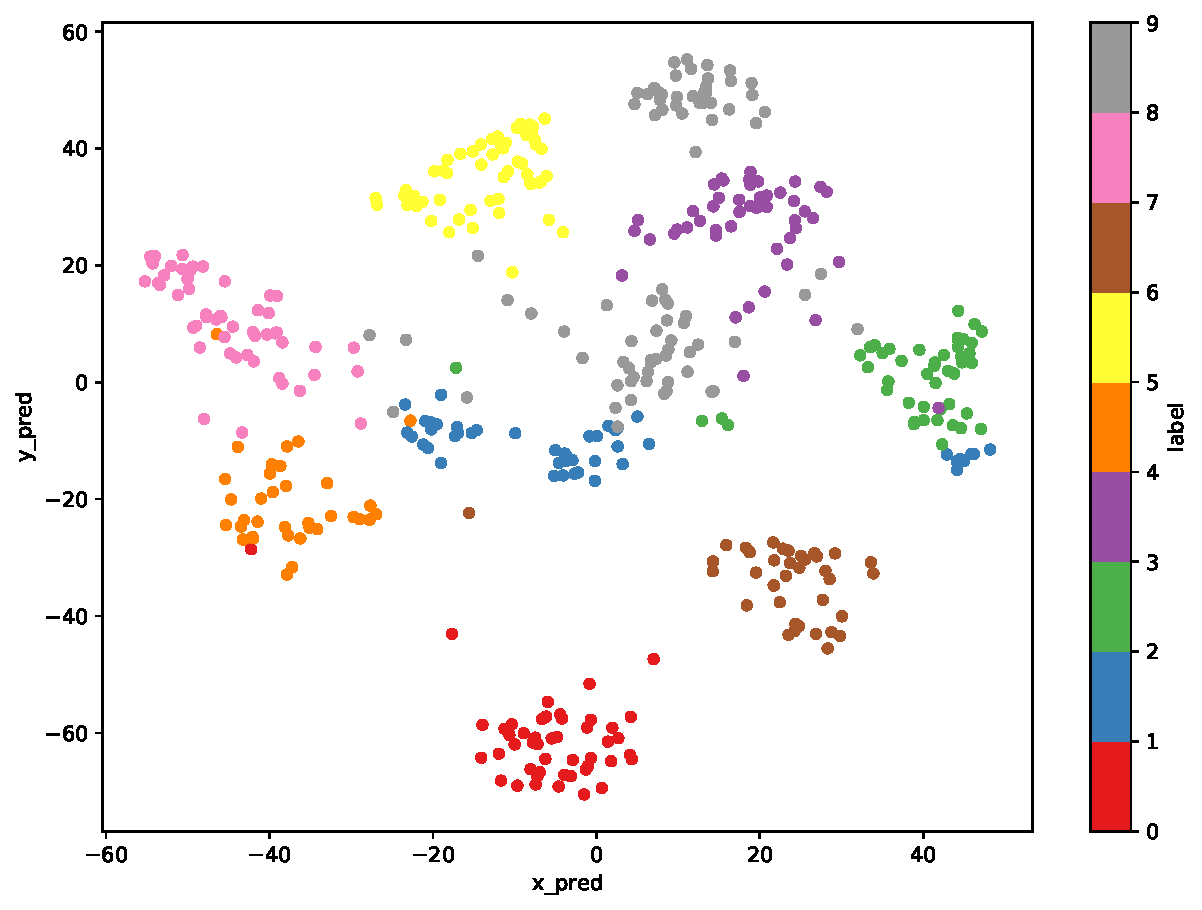
\includegraphics[width=12cm]{figures/app1plotpredictions.pdf}
\caption{\label{figureNN1}Low dimensional space from neural net trained for t-SNE.}
\end{figure}

\begin{figure}[p]
\centering
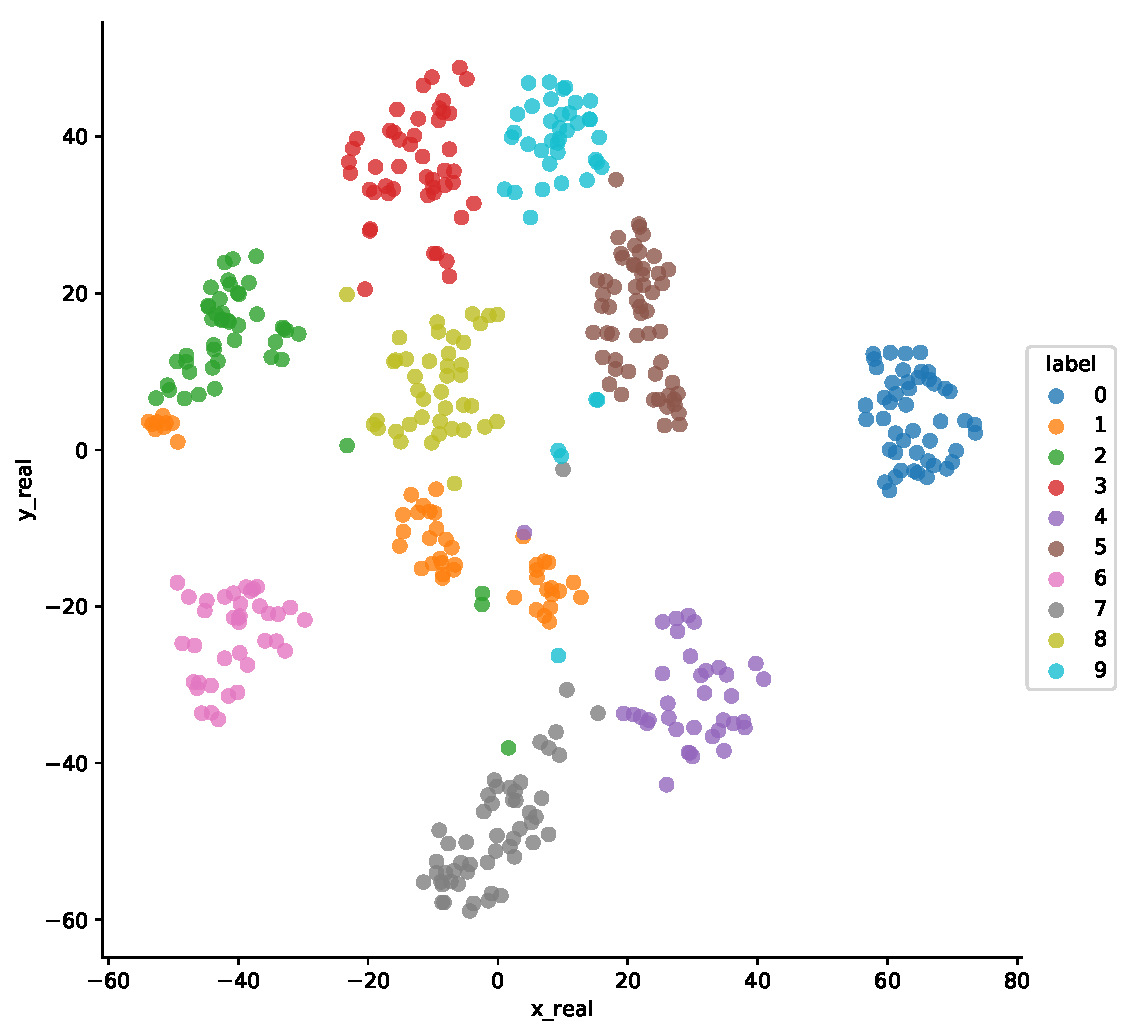
\includegraphics[width=12cm]{figures/app1plotreal.pdf}
\caption{\label{figureTSNE}Low dimensional space from t-SNE}
\end{figure}

\begin{figure}[p]
\centering
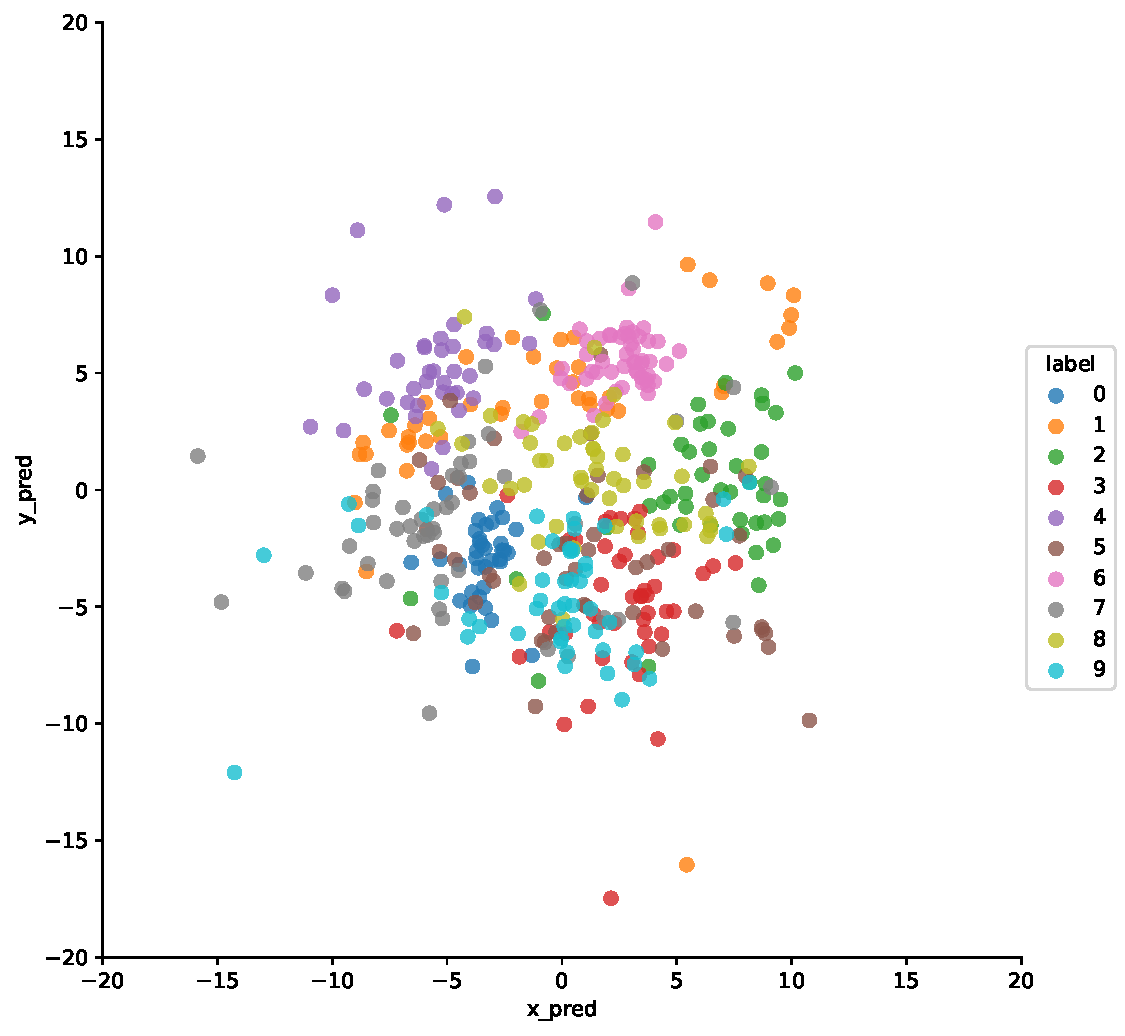
\includegraphics[width=12cm]{figures/app1plotpredictionsmds.pdf}
\caption{\label{figureNN2}Low dimensional space from neural net trained for MDS.}
\end{figure}

\begin{figure}[p]
\centering
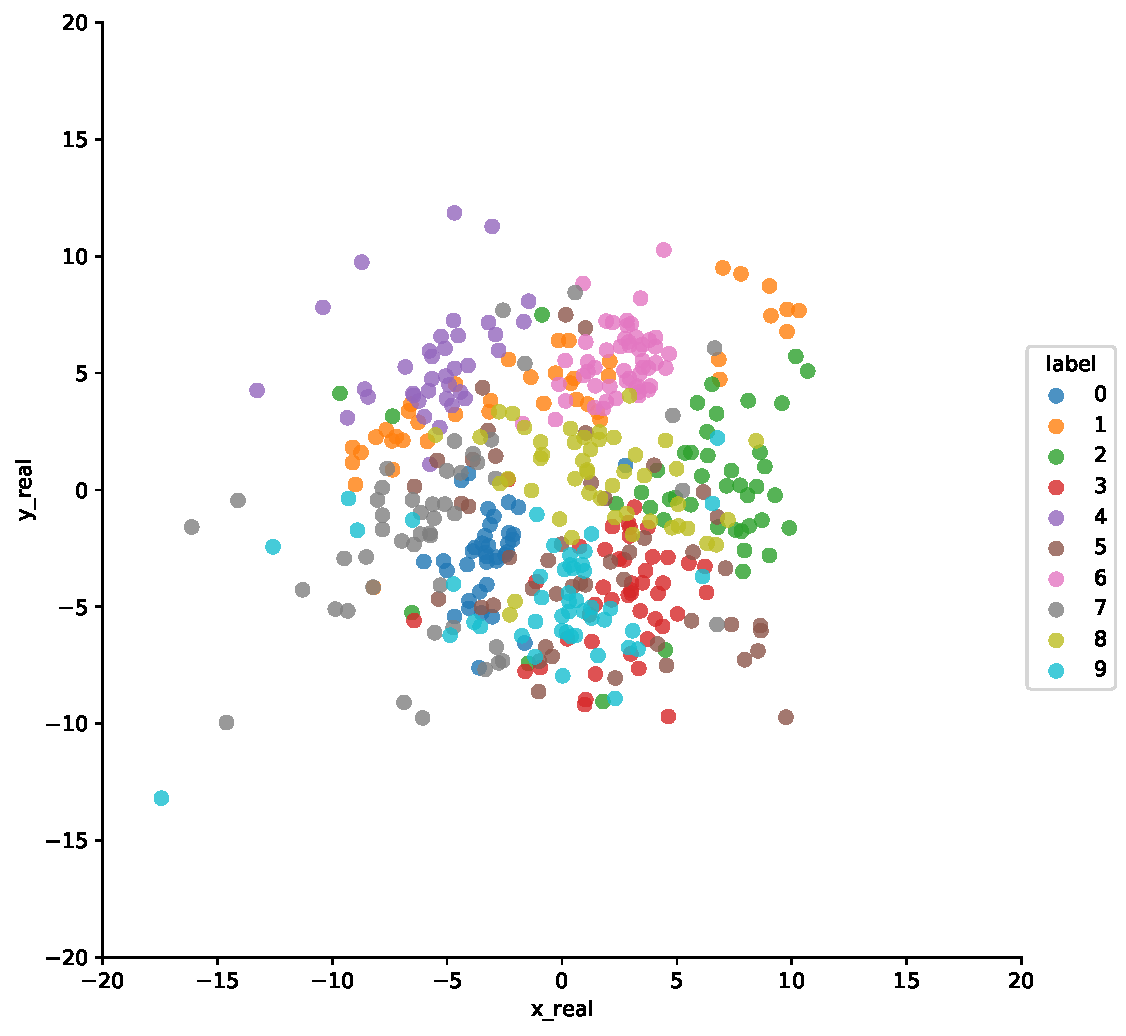
\includegraphics[width=12cm]{figures/app1plotrealmds.pdf}
\caption{\label{figureMDS}Low dimensional space from MDS}
\end{figure}

\newpage


\section{Framework 2: Approximate Nearest Neighbor search}
\label{sec:app2}

The second application consists in the computation of nearest neighbours in a low-dimensional space. This second implementation focuses on the Multidimensional Scaling algorithm, since this particular method's objective is to preserve distances and, consequently, local structure (in terms of neighbors) of the data. The aim is to compute the nearest neighbours in the output space and check how accurate this computation is compared to a brute force approach. Since this computation is performed in a lower dimensional space, it provides a real application with significant improvements in speed and memory usage, since we are only storing a reduced number of columns and performing euclidean distance computations using these dimensions.

\subsection{Algorithm: Approximate nearest neighbors using MDS embeddings}
\label{ssec:nneigh}

As it has just been stated, the main task contemplated in this application is the computation of nearest neighbours. The following tests bear with re-usability and time / memory usage reduction.

Regarding the first point, because of MDS being non-parametric, there is no way to obtain the embeddings for new samples. This means if we have already obtained the low-dimensional map of points from the dataset, it would be impossible to obtain the coordinates of a new sample unless the algorithm is recomputed again from scratch. If we based our nearest neighbours search in the output space from the MDS algorithm it's true that we would gain the benefits of making computations in a lower dimensional space.

Nearest neighbours brute force approach \citep{brute} is known to have poor scalability and both low CPU / memory efficiency since it requires to compute euclidean distances between each point and all of the rest and then sort them according to their distances, from lowest to highest. This means that its computational complexity order corresponds to the expression $O(N^{2})$, where $n$ is the number of samples of the query.

Since euclidean distances are computed as:

$$ dist(p,q) = \sqrt{(q_{1}-p_{1})^{2}+(q_{2}-p_{2})^{2}+ ... + (q_{n}-p_{n})^{2}} = \sqrt{\sum_{j=1}^{d} (q_{j}-p_{j})^{2}}$$

Therefore, if we increase the number of samples $n$, the amount of pairwise distance computations needed increases as $n^{2}$. The brute force algorithm's complexity in terms of number of dimensions and sample is consequently $O(N^{2}*D)$.

As for memory usage (complexity) and taking into account the previous ideas of how neighbours are computed, this model requires the original matrix to be stored which means the memory complexity also depends on the number of points and their dimensions, which corresponds to the following expression: $O(N*D)$. Our experimental approach tries to deal with these inconveniences by learning an unsupervised algorithm's map.

The algorithm involves two phases: one fitting process (algorithm \ref{alg2}) and afterwards its usage (transformation) for new points (algorithm \ref{alg3}). This is why the original dataset is split into two subsets, one for training and the second one to test out-of-sample performance.

The training phase aims to obtain all parameters or transformations which will be later used to transform the data. During the fitting process, the MDS computes the embeddings (vectors of all samples in the embedding space) directly by using gradient descent on its loss function (stress). This is why we would not be able to obtain the transformation of a new sample without having to fit the whole dataset again (which requires computational time), thus we would not be able to step into the process of computing nearest neighbours in the low-dimensional space unless we are querying already known samples.

Instead, in this proposal, and relative to the first application (\ref{sec:app1}), the training consists in learning the mapping of a dimensionality reduction algorithm from a high-dimensional space to a low-dimensional space by training a neural net to do so. In this case, the model just saves the neural net's parameters which replicate the MDS, instead of the exact transformations from it, and stores in memory only the embeddings (lower memory and size) of the training set. Then, when a new out of sample sample is queried, there is no need to compute the whole MDS algorithm to be able to transform the data because we have a neural net that can approximate the embedding operation.

Accordingly, the approximate nearest neighbours model designed will have its computational time and memory complexity reduced by the ratio between the original (\textit{d}) and the low-dimensional space's dimensions (\textit{k}). We shall also take into account that the higher the level of compression, the more the recall / precision will be degraded.

\begin{itemize}
\item Computational time complexity: $O(N^{2}*K)$
\item Memory complexity: $O(N*K)$
\end{itemize}

To conclude with, the overall procedure can be summarized in the following manner: when a new sample is queried (in order to find its k-nearest neighbours), it is firstly transformed by the neural net from \textit{d} dimensions to \textit{k}, corresponding to the low-dimensional space, by predicting with the parameters learned from MDS. This parameters are learned in cross-validation to ensure that test set samples are unseen. Finally, the K nearest neighbours are computed comparing in the low  dimensional space. The objective is to check whether these whole procedure is faster than a brute force approach. Memory usage is lower and this is a fact, since we only need to store a matrix with a reduced shape.

\vspace{25px}
\begin{algorithm}
\caption{Low dimensional nearest neighbours calculation}
\label{alg2}
\begin{algorithmic}[1]
\Procedure{Fitting process}{}
\State $\textit{\textbf{X}} \gets \text{imputed and standardized dataset}$
\State $\textit{\textbf{X\_mds}} \gets \text{compute MDS from \textit{\textbf{X}}}$
\BState \emph{neural net model construction}
\BState \emph{fit neural net model}
\BState \emph{save reduced matrix from training neural net}
\EndProcedure
\end{algorithmic}
\end{algorithm}
\hfill

\begin{algorithm}
\caption{Low dimensional nearest neighbours calculation}
\label{alg3}
\begin{algorithmic}[1]
\Procedure{NN calculation for new sample}{}
\State $\textit{\textbf{x}} \gets \text{new sample}$
\State $\textit{\textbf{x\_reduced}} \gets \text{predicted output from neural net with x (reduction)}$
\BState \emph{nearest neighbours calculation with brute force algorithm in the low dimensional space}
\EndProcedure
\end{algorithmic}
\end{algorithm}

\subsection{Results}
\label{ssec:res2}

\begin{itemize}
    \item Dataset
\end{itemize}

The dataset \textit{"forests.csv"} is used for this application and is obtained from the UCI Machine Learning Repository \citep{ucidata}. For convenience, a random subsample of 20.000 examples is selected with 55 features each. All features are numeric variables that describe several characteristics and measurements of each forest. The forest class is represented by a number in a range of 1 to 7, shaping the last column of the dataset.

The reason why this dataset is chosen for this particular application relies on the need to compute a substantial amount of examples in the training phase to obtain a reliable model and to be able to asses time and memory performance improvements and also recall/precision degradation.

\begin{itemize}
    \item Metrics
\end{itemize}

With this second implementation, the main metrics to look at correspond to precision and computational measurements, such as time and memory usage. As the objective is to compute nearest neighbours, precision is described as the percentage of nearest neighbours preserved in comparison to a brute force approach in the original space. In the case of time and memory, the measurements are strictly related to the algorithm's performance, thus we can compute how much time they require to find these neighbours and the memory needed.

The following tables (\ref{metrics21}, \ref{metrics22}, \ref{metrics23}) relate the model used to compute the neural net with the previous metrics, depending on the dimensions of the low-dimensional space chosen to lower the number of features.

\begin{table}[h]
\centering
\begin{tabular}{lrrrrr}
\toprule
{} &  \ npreserved &    t\_model &  t\_brute &  mem\_model &  mem\_brute \\
\midrule
model1 &     0.565350 &  0.771945 &  1.074873 &     112112 &   3080112 \\
model2 &     0.571843 &  0.785027 &  1.084613 &     112112 &   3080112 \\
model3 &     0.570347 &  0.800511 &  1.067814 &     112112 &   3080112 \\
model4 &     0.567003 &  0.755689 &  1.082235 &     112112 &   3080112 \\
model5 &     0.564130 &  0.796335 &  1.038609 &     112112 &   3080112 \\
model6 &     0.564723 &  0.808626 &  1.021288 &     112112 &   3080112 \\
model7 &     0.569093 &  0.767841 &  1.096126 &     112112 &   3080112 \\
model8 &     0.572430 &  0.922942 &  0.888819 &     112112 &   3080112 \\
\bottomrule
\end{tabular}

\caption{\label{metrics21}Nearest neighbours calculation in four dimensions}
\end{table}

\begin{table}[h]
\centering
\begin{tabular}{lrrrrr}
\toprule
{} &  \%npreserved &    nntime &  realtime &  mem\_model &  mem\_real \\
\midrule
model1 &     0.728400 &  0.993689 &  1.204910 &     224112 &   3080112 \\
model2 &     0.780377 &  0.969519 &  1.218967 &     224112 &   3080112 \\
model3 &     0.779553 &  0.971488 &  1.219617 &     224112 &   3080112 \\
model4 &     0.760667 &  0.974497 &  1.152932 &     224112 &   3080112 \\
model5 &     0.761370 &  0.978987 &  1.146578 &     224112 &   3080112 \\
model6 &     0.756977 &  0.990972 &  1.081272 &     224112 &   3080112 \\
model7 &     0.771057 &  0.972610 &  1.216437 &     224112 &   3080112 \\
model8 &     0.771207 &  1.006541 &  0.947692 &     224112 &   3080112 \\
\bottomrule
\end{tabular}

\caption{\label{metrics22}Nearest neighbours calculation in eight dimensions}
\end{table}

\begin{table}[h]
\centering
\begin{tabular}{lrrrrr}
\toprule
{} &  \ npreserved &    nntime &  realtime &  mem\_model &  mem\_real \\
\midrule
model1 &     0.669377 &  0.952179 &  1.175327 &     504112 &   3080112 \\
model2 &     0.855583 &  0.953779 &  1.175554 &     504112 &   3080112 \\
model3 &     0.837507 &  0.950562 &  1.197267 &     504112 &   3080112 \\
model4 &     0.848860 &  0.961237 &  1.126327 &     504112 &   3080112 \\
model5 &     0.844383 &  0.955949 &  1.114451 &     504112 &   3080112 \\
model6 &     0.835173 &  0.966225 &  1.045986 &     504112 &   3080112 \\
model7 &     0.855930 &  0.955785 &  1.174047 &     504112 &   3080112 \\
model8 &     0.853597 &  0.945284 &  0.928504 &     504112 &   3080112 \\
\bottomrule
\end{tabular}

\caption{\label{metrics23}Nearest neighbours calculation in eighteen dimensions}
\end{table}

The approximate algorithm hereby proposed can also be compared to other approximate nearest neighbours algorithms such as KD-Tree \citep{kdtree}. KD-Tree is a binary tree that creates divisions of the space using splitting planes which are orthogonal to the axis. Each node has a corresponding region called cell and the root's cell has to include all the samples in the dataset. For each region we have a hyper-plane that divides the subspace in two regions. This is recursively repeated until there are no points left or a minimum of samples per leaf is reached. This model works well for datasets with a moderate / small number of dimensions but has no memory improvements. Its computational complexity is  $O(NlogN)$. However, when the number of dimensions increase, the behaviour tends to get worse. For small datasets, query times may be even worse than brute force, but its scalability is significantly better. Table \ref{metrics24} corresponds to the first dataset of the application.

\begin{table}[h]
\centering
\begin{tabular}{lrrrrr}
\toprule
{} &  \%npreserved &    nntime &  realtime &  mem\_model &  mem\_real \\
\midrule
model1 &          1.0 &  2.599825 &  1.173718 &    3080112 &   3080112 \\
model2 &          1.0 &  2.633631 &  1.157942 &    3080112 &   3080112 \\
model3 &          1.0 &  2.624684 &  1.168484 &    3080112 &   3080112 \\
model4 &          1.0 &  2.613410 &  1.153366 &    3080112 &   3080112 \\
model5 &          1.0 &  2.614144 &  1.169271 &    3080112 &   3080112 \\
model6 &          1.0 &  2.609788 &  1.184947 &    3080112 &   3080112 \\
model7 &          1.0 &  2.637135 &  1.164681 &    3080112 &   3080112 \\
model8 &          1.0 &  2.612835 &  1.174181 &    3080112 &   3080112 \\
\bottomrule
\end{tabular}

\caption{\label{metrics24}KD-Tree computing nearest neighbours}
\end{table}

Although the total amount of neighbours are preserved by KD-tree, both the computational time and memory used by the model are high, two times compared to brute force algorithm. The next two tables (\ref{metrics25} and \ref{metrics26}) compare the approximate model and the kd-tree approximate nearest neighbours computation with a new dataset that has 4000 instances and 281 features per sample.

\begin{table}[h]
\centering
\begin{tabular}{lrrrrr}
\toprule
{} &  npreserved &   t\_model &   t\_brute &  mem\_model &  mem\_brute \\
\midrule
model1 &     0.30045 &  0.152567 &  0.206344 &    1200112 &    6744112 \\
model2 &     0.43732 &  0.140289 &  0.172093 &    1200112 &    6744112 \\
model3 &     0.38892 &  0.139835 &  0.178780 &    1200112 &    6744112 \\
model4 &     0.46497 &  0.132087 &  0.177754 &    1200112 &    6744112 \\
model5 &     0.41835 &  0.132285 &  0.173796 &    1200112 &    6744112 \\
model6 &     0.49443 &  0.133642 &  0.174198 &    1200112 &    6744112 \\
model7 &     0.50684 &  0.136121 &  0.174210 &    1200112 &    6744112 \\
model8 &     0.59107 &  0.136980 &  0.184086 &    1200112 &    6744112 \\
\bottomrule
\end{tabular}

\caption{\label{metrics25}Nearest neighbours calculation in 100 dimensions from new dataset}
\end{table}

\begin{table}[h]
\centering
\begin{tabular}{lrrrrr}
\toprule
{} &  npreserved &   t\_kdtree &   t\_brute &  mem\_kdtree &  mem\_brute \\
\midrule
model1 &     0.99992 &  2.211247 &  0.383505 &   13808037 &    6744112 \\
model2 &     0.99992 &  2.088237 &  0.442901 &   13808037 &    6744112 \\
model3 &     0.99992 &  1.973441 &  0.446145 &   13808037 &    6744112 \\
model4 &     0.99992 &  1.844881 &  0.388873 &   13808037 &    6744112 \\
model5 &     0.99992 &  2.136054 &  0.422400 &   13808037 &    6744112 \\
model6 &     0.99992 &  1.878483 &  0.433052 &   13808037 &    6744112 \\
model7 &     0.99992 &  2.173580 &  0.405178 &   13808037 &    6744112 \\
model8 &     0.99992 &  1.897629 &  0.438579 &   13808037 &    6744112 \\
\bottomrule
\end{tabular}

\caption{\label{metrics26}KD-Tree computing nearest neighbours from new dataset}
\end{table}

The computational time KD-Tree requires is twelve times the computational time from the approximate model in the best of the cases. The memory KD-Tree needs to compute its operations is nearly also twelve times more than for the model designed in this experiment.

\subsection{Conclusion}
\label{ssec:conc2}

Computing nearest neighbours in nowadays applications has become an important issue. The need to report them live (for instance for advertisement recommendation) demands new state-of-the-art algorithms like the model previously proposed. It consists in lowering the sample's dimensions with a neural net which has learned how to replicate a MDS, and then, nearest neighbours are computed in the low-dimensional space.

As seen in the results studied before, there is a clear relation between precision obtained and time and memory usage. We can sacrifice a bit of recall and get huge improvements in memory usage, which can reduce application costs considerably.

Although KD-Tree also uses the idea of creating a non linear kernel, regarding precision, time and memory usage this gets higher when a complex dataset is provided, and it has no benefits regarding memory usage. 

The computational complexities for the three algorithms studied are the next ones (taking into account dimensions computed):

\begin{itemize}
\item Brute force algorithm: $ O(N^{2} * D)$ 
\item KD-Tree algorithm: $ O(NlogN * D)$ 
\item Approximate nearest neighbours algorithm: $ O(N^{2}*D^{*}) = O(N^{2}*\frac{D}{3})$ 
\end{itemize}

The following figure illustrates computational complexities for an increasing number of dimensions:

\begin{figure}[h]
\centering
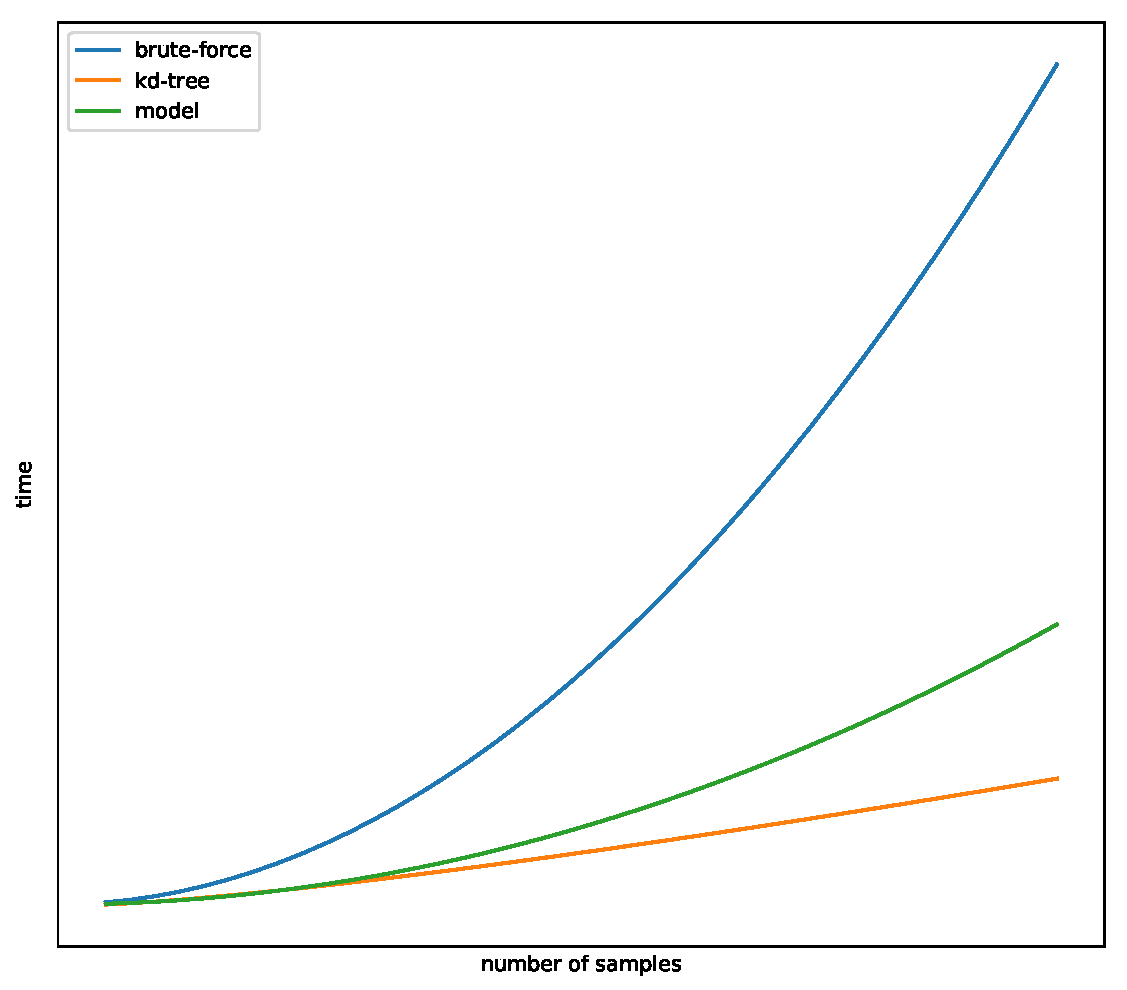
\includegraphics[width=12cm]{figures/complexities.pdf}
\caption{\label{figurecomplexities}Algorithms' complexities.}
\end{figure}




%%%%%%%%%%%%%%%%%%%%%%%%%%%%%%%%%%%%%%%%%%%%%%%%%%%%%%%%%%%%%%%%

%-----------------------------------------------------
% Chapter: Conclusion
%-----------------------------------------------------

\chapter{Conclusions and Future Work}
\label{chap:conc}

Dimensionality reduction algorithms are commonly used for a wide number of applications, such as data compression, feature decorrelation, model improvement, visualization and many more. Classic compression algorithms such as PCA are often used as part of machine learning pipelines (for supervised problems) and have some advantages (linearity, interpretability and simplicity) but they have rigid assumptions and a considerable bias when looking at the structure of the data. 

We took an in depth look at some of the new state-of-the art algorithms that aim to derive space transformations (sometimes called manifold methods) and can better preserve the local and global structure of the data. These are incredibly powerful both for visualization and as general compression techniques. However, a big number of these algorithms are based on one-off optimizations (mainly gradient descent over fancy cost functions) on a sample set and can therefore be run only once. This means that, although being more powerful, they are not reusable and sometimes end up being useless for real applications, as it is impractical to constantly re-run these algorithms when new samples need to be analyzed.

We propose a novel technique that makes use of wide non-regularized neural nets with multi-output and a custom euclidean distance loss that can learn pretty much any of these manifold (dimensionality reduction) methods. This framework allows us to re-use and deploy any embedding algorithms with great speed, accuracy, efficiency and low memory usage (we just need to store the net's parameters). We also showed two real applications including an approximate nearest neighbors algorithm using MDS and a replicating neural net. 

These reduction algorithms have many more applications though. They can be even used as a feature engineering technique for model stacking. Kagglers have often suggested that adding manifold coordinates as new features to a sample set can suddenly make a model stack improve. This technique, however, was useless for real ensembles since the manifold features could not be included during live prediction. In the future, we look forward to explore more applications of this framework such as the latter and improve the flexibility of the classes defined with more options and a more generic API.

%-----------------------------------------------------
% Chapter: Code
%-----------------------------------------------------

\chapter{Appendix}
\label{chap:appendix}
\nocite{*}

\section{Code: Application 1}
\label{code1}

By running the following python 3 code these results can be easily reproduced. For better performance, a server with multiple cores (and possibly a GPU) may be used, since all tests have been parallelized using python 3's \textbf{joblib} package.

\vspace{10px}
\inputminted[baselinestretch=1, fontsize=\scriptsize, breaklines]{python}{application1.py}
\newpage

\section{Code: Application 2}
\label{code2}

\inputminted[baselinestretch=1, fontsize=\scriptsize, breaklines]{python}{application2.py}
\newpage

\section{Code: Python classes}
\label{codeclasses}

The following python classes are compatible with the \textit{Scikit-Learn} API and can be used along with \textit{Keras} and \textit{Tensorflow} to replicate any unsupervised algorithm. These classes were also tested for other algorithms such as PCA, Isomap, Locally Linear Embeddings and others, and gave extremely good results in all cases. It allows for a flexible and scalable definition of the neural net structure and can be easily integrated in machine learning pipelines (such as the ones in the Scikit Learn API) and deployed in a real application.

Using these classes one would be able to build an application such as the following: using Tf-IDF representations of random texts we could train a t-SNE and create a 2D visualization of these texts where close texts would have a clear semantic similarity. We could even cluster these texts in this low dimensional space and discover the semantic properties of all zones in it. Then by using a replicator class, we can train a neural net to learn the t-SNE embeddings and be able to visualize the semantic properties of any given text pasted by the user in the application.

\inputminted[baselinestretch=1, fontsize=\scriptsize, breaklines]{python}{classes.py}


%-----------------------------------------------------
% Chapter: Bibliography
%-----------------------------------------------------

\label{chap:bib}
\addcontentsline{toc}{chapter}{Bibliography}
\bibliography{mybib}
\nocite{*}

% %%%%%%%%%%%%%%%%%%%%%%%%%%%%
% % BIBLIOGRAPHY
% \clearpage
% \phantomsection
% \addcontentsline{toc}{chapter}{Bibliography}
% \bibliography{bib}
% %%%%%%%%%%%%%%%%%%%%%%%%%%%%


%%%%%%%%%%%%%%%%%%%%%%%%%%%%
% END DOCUMENT
\end{document}
%%%%%%%%%%%%%%%%%%%%%%%%%%%%